\documentclass[11pt,fleqn]{article}
\usepackage{../cs70,latexsym,epsf, amsmath,amsfonts,graphicx,url}
\lecture{13}
\def\title{Note \the\lecturenumber}
\begin{document}
\maketitle

\section*{Introduction to Discrete Probability}

In the last note we considered the probabilistic experiment where we flipped a fair coin $10,000$ times
and counted the number of Hs. We asked "what is the chance that we get between $4900$ and $5100$ 
Hs". One of the lessons was that the remarkable concentration of the fraction of Hs had something to do 
with the astronomically large number of possible outcomes of $10,000$ coin flips. 

In this note we will formalize all these notions for an arbitrary probabilistic experiment. We will start by 
introducing the space of all possible outcomes of the experiment, called a sample space. Each element 
of the sample space is assigned a probability - which tells us how likely it is to occur when we actually 
perform the experiment. The mathematical formalism we introduce might take you some time to get 
used to. But you should remember that ultimately it is just a precise way to say what we mean when we
describe a probabilistic experiment like flipping a coin $n$ times.

\section*{Random Experiments}
In general, a probabilistic experiment consists of drawing a sample of $k$ elements from a 
set $S$ of cardinality $n$. The possible outcomes of such an experiment are exactly the 
objects that we counted in the last note. Recall from the last note that we considered four
possible scenarios for counting, depending upon whether we sampled with or without 
replacement, and whether the order in which the $k$ elements are chosen does or does
not matter. The same will be the case for our probabilistic experiments. 
The outcome of the random experiment is called a
{\em sample point}. The
{\em sample space}, often denoted by $\Omega$, is the set of all
possible outcomes. 

An example of such an
experiment is tossing a coin $4$ times.
In this case, $S = \{H,T\}$ and we are drawing
4 elements with replacement.
$HTHT$ is an example of a sample point and
the sample space has $16$
elements:

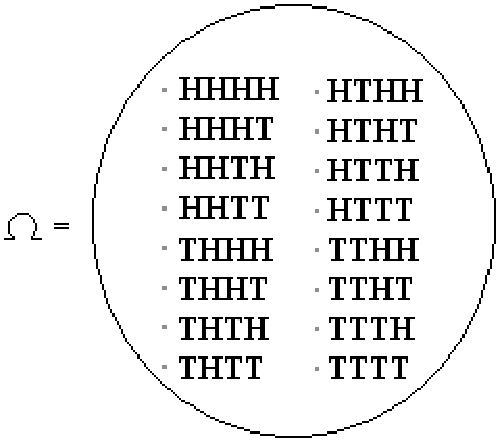
\includegraphics[bb = -80 0 0 218, scale = 0.7]{samplespace}

How do we determine the chance of each particular outcome, such as $HHT$, of our experiment?
In order to do this,
we need to define the probability for each sample point, as we will do below. 

\section*{Probability Spaces}


A \underline{probability space} is a sample space~$\Omega$, together with
a \underline{probability} $\Pr[\omega]$ for each sample point~$\omega$, such
that
\begin{itemize}
\item $0\le\Pr[\omega]\le 1$ for all $\omega\in\Omega$.
\item $\displaystyle\sum_{\omega\in\Omega}\Pr[\omega] = 1$, i.e., the sum of
the probabilities of all outcomes is~1.
\end{itemize}

The easiest way to assign probabilities to sample points is
uniformly: if $|\Omega| = N$,
then $\Pr[x] = \frac{1}{N}$ $\forall x \in \Omega$. 
For example, if we toss a fair coin 4 times,
each of the 16 sample points (as pictured above) is assigned
probability $\frac{1}{16}$. We will see examples of non-uniform
probability distributions soon.

After performing an experiment, we are often
interested in knowing whether an event occurred. 
For example, we might be interested in the event that there were
``exactly 2 $H$'s in four tosses of the coin". How do we formally define
the concept of an event in terms of the sample space $\Omega$?
Here is a beautiful answer. We will identify the event ``exactly 2 $H$'s in four tosses of the coin"
with the subset consisting of those outcomes in which there are exactly two H's: \\
$\{HHTT, HTHT, HTTH, THHT, THTH, TTHH\} \subseteq \Omega$.
Now we turn this around and say that formally an \underline{event} $A$ is just a subset of the sample space,
$A \subseteq \Omega$. 

How should we define the probability of an event~$A$?  Naturally,
we should just {\it add up\/} the probabilities of the sample points in~$A$.

For any event $A \subseteq \Omega$, we define the \underline{probability of~$A$}
to be $$
   \Pr[A] = \sum_{\omega\in A} \Pr[\omega].  $$

Thus the probability of getting exactly two $H$'s in four coin tosses
can be calculated using this definition as follows. $A$ consists of all
sequences that have exactly two $H$'s, and so $|A| ={4\choose 2}= 6$. 
For this example, there are $2^4 = 16$ possible outcomes for flipping four coins. 
Thus, each sample point $\omega \in A$ has probability $\frac{1}{16}$; and, as 
we saw above, there are six sample points in~$A$, giving us
$\Pr[A] = 6 \cdot \frac{1}{16} = \frac{3}{8}$.

\section*{Examples}

We will now look at examples of random experiments and 
their corresponding sample spaces, along with possible probability spaces and events. 

\subsection*{Coin Flipping}
Suppose we have a coin of bias $p$, and our experiment consists of flipping the coin $4$ times. 
The sample space $\Omega$ consists of the sixteen possible sequences of H's and T's shown 
in the figure on the last page. 

The probability space depends on $p$. If $p = \frac{1}{2}$ the probabilities are assigned uniformly; the probability
of each sample point is $\frac{1}{16}$. What if the coin comes up heads with
probability $\frac{2}{3}$ and tails with probability $\frac{1}{3}$ (i.e. the bias is $p = \frac{2}{3}$)?
Then the probabilities are different. 
For example,
$\Pr[HHHH]={2\over 3}\times{2\over 3}\times{2\over 3}\times{2\over 3}={16\over{81}}$,
while $\Pr[TTHH]={1\over 3}\times{1\over 3}\times{2\over 3}\times{2\over 3}={4\over{81}}$.
[{\it Note: We have cheerfully\/ {\rm multiplied} probabilities here;
we'll explain why this is OK later.  It is\/ {\rm not} always OK!\/}]

What type of events can we consider in this setting? Let event $A$ be the event that 
all four coin tosses are the same. Then $A = \{HHHH,TTTT\}$. 
$HHHH$ has probability ${2\over 3}^4$ and $TTTT$ has probability 
${1\over 3}^4$. Thus, $\Pr[A] = \Pr[HHHH] + \Pr[TTTT] = {2\over 3}^4 + {1\over 3}^4 = {17\over{81}}$. 

Next, consider event $B$: the event that there are exactly two heads. The probability
of any particular outcome with two heads (such as $HTHT$) is ${2\over 3}^2 {1\over 3}^2$. 
How many such outcomes are there? There are ${4\choose 2}=6$
ways of choosing the positions of the heads, and these choices
completely specify the sequence.  So $\Pr[B]=6{2\over 3}^2 {1\over 3}^2 = {24\over{81}}= {8\over{27}}$. 

More generally, if we flip the coin $n$ times, 
we get a sample space $\Omega$ of cardinality~$2^n$. The sample points are all possible sequences of $n$ H's and T's. 
If the coin has bias $p$, and if we consider any sequence of $n$ coin flips with exactly $r$ H's,
then the the probability of this sequence is $p^r(1-p)^{n-r}$. 

Now consider the event $C$ that we get exactly $r$ H's when we flip the coin $n$ times. 
This event consists of exactly ${n \choose r}$ sample points. Each has probability $p^r(1-p)^{n-r}$.
So the probability of this event, $P[C] = {n \choose r}p^r(1-p)^{n-r}$.

Biased coin-tossing sequences show up in many contexts:
for example, they might model the behavior of $n$ trials of a faulty system,
which fails each time with probability~$p$.

\subsection*{Rolling Dice}

The next random experiment we will discuss consists of rolling two dice.
In this experiment, 
$\Omega=\{(i,j):1\le i,j\le 6\}$.  The probability space is \underline{uniform}, i.e.
all of the sample points have the {\it same\/} probability, which must be $1\over{|\Omega|}$.
In this case, $|\Omega| = 36$, so each sample point has probability $\frac{1}{36}$.
In such circumstances, the
probability of any event~$A$ is clearly just$$
\Pr[A] = { \hbox{\rm \# of sample points in $A$} \over
\hbox{\rm \# of sample points in $\Omega$} }
= {{|A|}\over{|\Omega|}}.  $$
So for uniform spaces, computing probabilities reduces to
{\it counting\/} sample points!

Now consider two events: the event $A$ that the sum of the dice is at least 10
and the event $B$ that there is at least one 6. By writing out the number of sample points
in each event, we can determine the number of sample points in each event; $|A| = 6$ and $|B| = 11$.
By the observation above, it follows that $\Pr[A] = \frac{6}{36} = \frac{1}{6}$ and $\Pr[B] = \frac{11}{36}$. 

\subsection*{Card Shuffling}
The random experiment consists of shuffling a deck of cards. $\Omega$ is equal to 
the set of the $52!$
permutations of the deck. The probability space is uniform.  
Note that we're really talking about an idealized mathematical
model of shuffling here; in real life, there will always be a bit of
bias in our shuffling.  However, the mathematical model is close enough
to be useful.

\subsection*{Poker Hands}
Here's another experiment: shuffling a deck of cards and dealing a poker hand.  In this case, $S$
is the set of 52 cards and 
our sample space $\Omega = \{$all possible poker hands$\}$, which corresponds
to choosing $k=5$ objects without replacement from a set of size $n=52$
where order does not matter.  Hence, as we saw in the previous Note,
$|\Omega| = {52 \choose 5} = \frac{52 \times 51 \times 50 \times 49 \times 48}{5 \times 4 \times 3 \times 2 \times 1} = 2,598,960$.
Since the deck is assumed to be randomly shuffled, the probability of each outcome is equally likely
and we are therefore dealing with a uniform probability space. 

Let $A$ be the event that the poker hand is a flush. 
[For those who are not addicted to gambling, a {\it flush\/}
is a hand in which all cards have the same suit, say Hearts.]
Since the probability space is uniform, computing $\Pr[A]$ reduces
to simply computing $|A|$, or the number of poker hands which are flushes.
There are 13 cards in
each suit, so the number of flushes in each suit is
${13}\choose 5$.  The total number of flushes is therefore
$4\cdot{{13}\choose 5}$.  Then we have  $$
               \Pr[\hbox{\rm hand is a flush}] =
                    {{4\cdot{{13}\choose 5}}\over{{{52}\choose 5}}} =
                    {{4\cdot{13!}\cdot 5!\cdot{47!}}\over{5!\cdot 8!\cdot{52!}}} =
                    {{4\cdot 13\cdot 12\cdot 11\cdot 10\cdot 9}\over
                                {52\cdot 51\cdot 50\cdot 49\cdot 48}}\approx
                    0.002.  $$

\subsection*{Balls and Bins}
In this experiment, we will throw 20 (labeled) balls into 10 (labeled) bins.
Assume that each ball is equally likely to land in any bin, regardless of what happens to
the other balls. 

If you wish to understand this situation in terms of sampling a sequence of $k$ elements 
from a set $S$ of cardinality $n$: here the set $S$ consists of the $10$ bins, and we are 
sampling with replacement $k= 20$ times. The order of sampling matters, since the balls 
are labeled. 

The sample space $\Omega$ is equal to 
$\{(b_1,b_2,\ldots,b_{20}):1\le b_i\le 10\}$, where the
component~$b_i$ denotes the bin in which ball~$i$ lands. The cardinality of
the sample space, $|\Omega|$, is equal to $10^{20}$- each element $b_i$ in the sequence
has 10 possible choices, and there are 20 elements in the sequence. More generally,
if we throw $m$ balls into $n$ bins, we have a sample space of size $n^m$. 
The probability space is uniform; as we said earlier, each ball is equally likely
to land in any bin. 

Let $A$ be the event that bin 1 is empty. Since the probability space is uniform, we simply
need to count how many outcomes have this property. This is 
exactly the number of ways all 20 balls can fall into the remaining nine bins, which is $9^{20}$. 
Hence, $\Pr[A]={{9^{20}}\over{{10}^{20}}}=({{9\over{10}}})^{20}\approx 0.12$.

Let $B$ be the event that bin 1 contains at least one ball. This event is the {\it complement\/} $\bar{A}$ of $A$, i.e., 
it consists of precisely those sample points which are not in $A$. So $\Pr[B] = 1 - \Pr[A] \approx .88$. 
More generally, if we throw $m$ balls into $n$ bins, we have: $$
               \Pr[\hbox{\rm bin 1 is empty}]=\left({{n-1}\over n}\right)^m=
                            \left({1-{1\over n}}\right)^m.  $$

As we shall see, balls and bins is another
probability space that shows up very often in Computer Science:
for example, we can think of it as modeling a load balancing
scheme, in which each job is sent to a random processor.

It is also a more general model for problems we have previously considered.
For example, flipping a fair coin 3 times is a special case in which the number of balls 
($m$) is 3 and the number of bins ($n$) is 2. Rolling two dice is a special case in which 
$m = 2$ and $n = 6$. 


\subsection*{Birthday Paradox}

The ``birthday paradox'' is a remarkable phenomenon that examines the chances that two people in a group
have the same birthday.  It is a ``paradox'' not because of a logical contradiction, but because it goes
against intuition. For ease of calculation, we take the number of days in a year to be 365. Then $U = \{1,\dots,365\}$,
and the random experiment consists of drawing a sample of $n$ elements from $U$, where the
elements are the birth dates of $n$ people in a group. Then $|\Omega| = 365^n$.
This is because each sample point is a sequence of possible birthdays for $n$ people; so there are $n$ points
in the sequence and each point has 365 possible values. 

Let $A$ be the event that at least two people have the same birthday. If we want to determine $\Pr[A]$,
it might be simpler to instead compute the probability of the complement of $A$, $\Pr[\bar{A}]$. $\bar{A}$ 
is the event that no two people have the same birthday.
Since $\Pr[A] = 1 - \Pr[\bar{A}]$, we can then easily compute $\Pr[A]$. 

We are again working in a uniform probability space, so we just need to determine $|\bar{A}|$. Equivalently, 
we are computing the number of ways there are for no two people to have the same birthday. There are 
365 choices for the first person,
364 for the second, \ldots, $365-n+1$ choices for the $n^{th}$ person, for a total of
$365 \times 364 \times \cdots \times (365-n+1)$.  Note that this is simply an application of 
the first rule of counting; we are sampling without replacement and 
the order matters. 

Thus we have $\Pr[{\bar A}] = \frac{|{\bar A}|}{|\Omega|} =
\frac{365 \times 364 \times \cdots \times (365-n+1)}{365^n}$. Then
$\Pr[A] = 1 - \frac{365 \times 364 \times \cdots \times (365-n+1)}{365^n}$.  This allows
us to compute $\Pr[A]$ as a function of the number of people,~$n$.  Of course, as $n$ increases
$\Pr[A]$ increases.  In fact, with $n=23$ people you should be willing to bet that at least
two people do have the same birthday, since then $\Pr[A]$ is larger than 50\%! For $n=60$
people, $\Pr[A]$ is over 99\%.

\section*{The Monty Hall Problem}

In an (in)famous 1970s game show hosted by one Monty Hall, a
contestant was shown three doors; behind one of the doors was a
prize, and behind the other two were goats.  The contestant picks
a door (but doesn't open it). Then Hall's assistant (Carol),
opens one of the other two doors, revealing a goat (since
Carol knows where the prize is, she can always do this).
The contestant is then given the option
of sticking with his current door, or switching to the other unopened one.
He wins the prize if and only if his chosen door is the correct one.
The question, of course, is: Does the contestant have a better chance
of winning if he switches doors?

Intuitively, it seems obvious that since there are only two remaining
doors after the host opens one, they must have equal probability. So
you may be tempted to jump to the conclusion that it should not matter
whether or not the contestant stays or switches. 

Yet there are other people whose intuition cries out that the contestant 
is better off switching. So who's correct? 

As a matter of fact, the contestant has a better chance of picking the car if he uses
the switching strategy. How can you convince yourself that this is true? 
One way you can do this is by doing a rigorous analysis. You would 
start by writing out the sample space, and then assign probabilities to 
each sample point. Finally you would calculate the probability of the 
event that the contestant wins under the sticking strategy. This is an 
excellent exercise if you wish to make sure you understand the formalism 
of probability theory we introduced above. 

Let us instead give a more intuitive pictorial argument. Initially when the 
contestant chooses the door, he has a $\frac{1}{3}$ chance of picking the car.
This must mean that the other
doors combined have a $\frac{2}{3}$ chance of winning. But after Carol opens
a door with a goat behind it, how do the probabilities change? Well,
everyone knows that there is a goat behind one of the doors that the
contestant did not pick. So no matter whether the contestant is winning or 
not, Carol is always able to open one of the other doors to reveal a goat. 
This means that the contestant still has a $\frac{1}{3}$ chance of winning. 
Also the door that Carol opened has no chance of winning. What about the last door? It must
have a $\frac{2}{3}$ chance of containing the car, and so the contestant has a higher
chance of winning if he or she switches doors. This argument can be summed up nicely
in the following picture:

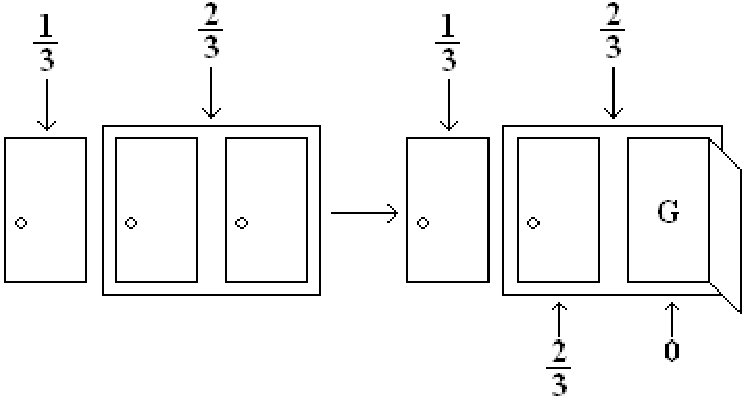
\includegraphics[bb = -40 0 0 190, scale=0.7]{monty}

You will be able to formalize this intuitive argument once we cover conditional probability. 

In the meantime, to approach this problem formally, first determine the sample space
and the probability space. Just a hint: it is not a uniform probability space!
Then formalize the event we have described above (as a subspace
of the sample space), and compute
the probability of the event. Good luck!

\section*{Summary}
The examples above illustrate the importance
of doing probability calculations systematically, rather than
``intuitively."  Recall the key steps in all our calculations:
\begin{itemize}
\item What is the \underline{sample space} (i.e., the experiment and its set of
possible outcomes)?
\item What is the \underline{probability} of each outcome (sample point)?
\item What is the \underline{event} we are interested in (i.e., which subset
of the sample space)?
\item Finally, compute the probability of the event by adding up
the probabilities of the sample points inside it.
\end{itemize}
Whenever you meet a probability problem, you should always go back
to these basics to avoid potential pitfalls.  Even experienced
researchers make mistakes when they forget to do this --- witness
many erroneous ``proofs'', submitted by mathematicians to newspapers
at the time, of the fact that the switching strategy in the Monty
Hall problem does not improve the odds.
\end{document}


